\documentclass[11pt]{scrartcl}
\usepackage{dominatrix}
\usepackage{solarized-light}
\lstset{
language=python
}

\renewcommand\thesection{Problem \arabic{section}}
\renewcommand\thesubsection{\arabic{section} (\alph{subsection})}
\renewcommand\thesubsubsection{(\roman{subsubsection})}
\DeclareMathOperator{\AU}{AU}
\DeclareMathOperator{\arcsec}{arcsec}
\DeclareMathOperator{\pc}{pc}
\DeclareMathOperator{\km}{km}
\DeclareMathOperator{\cm}{cm}
\DeclareMathOperator{\rad}{rad}
\DeclareMathOperator{\s}{s}
\DeclareMathOperator{\degrees}{degrees}
\DeclareMathOperator{\degree}{degree}
\DeclareMathOperator{\arcmin}{arcmin}

\newcommand\pow[2]{\ensuremath{#1 \times 10^{#2}}}

\title{Problem Set 1 Solutions}
\subject{ASTR 1404 Stars, Galaxies, and Cosmology}
%\author{James H. Applgate}
\begin{document}
\maketitle

\section{}

One full circle is $2\pi \rad$ and $360$ degrees. Thus the number of degrees in a $\rad$ is:

\[1\ \text{Circle} = 2\pi \rad = 360\degrees\]

Then,

\[1 \rad = \frac{360}{2\pi}\degrees\]

\subsection{}

\[1 \rad = 57.3\degrees\]

\subsection{}

\begin{align*}
1\degree &= 60\arcmin \\
1 \rad &= \frac{360}{2\pi} \degrees = \frac{360}{2\pi} \times 60 \arcmin \\
1 \rad &= \pow{3.44}{3}\arcmin
\end{align*}

\subsection{}

\begin{align*}
1\arcmin &= 60\arcsec \\
1 \rad &= \pow{3.44}{3}\arcmin = (\pow{3.44}{3})\times(60)\arcsec \\
1 \rad &= \pow{2.06}{5}\arcsec
\end{align*}

\subsection{}

\begin{align*}
1 \degree &= \frac{2\pi}{360}\rad \\
1 \degree &= 0.0175 \rad = {1.75}{-2}\rad
\end{align*}

\subsection{}

\begin{align*}
1 \arcmin &= \frac{1}{60}\deg \\
1 \arcmin &= \frac{2\pi}{360} \times \frac{1}{60} \rad \\
1 \arcmin &= \pow{2.91}{-4}\rad
\end{align*}

\subsection{}

\begin{align*}
1 \arcmin &= \pow{2.91}{-4}\rad \\
1 \arcsec &= \frac{1}{60}\arcmin = \pow{2.91}{-4} \times \left(\frac{1}{60}\right) \rad \\
1 \arcsec &= \pow{4.85}{06}\rad
\end{align*}


\section{}

The angular separation of the Earth-Moon system as seen from the Sun is

\begin{align*}
\theta &=\frac{\text{Earth-Moon distance}}{1\AU} \\
&= \frac{\pow{3.84}{10}\cm}{\pow{1.5}{13}\cm} \\
&= \pow{2.56}{-3}\rad \\
&= 0.147 \degrees = 8.8\arcmin
\end{align*}

Remember that $1\AU = \pow{1.5}{13}\cm$ and $D_M = 384,000\km = \pow{3.84}{10}\cm$


\section{}

\subsection{}

\begin{align*}
\theta_J &= \frac{D_J}{4\AU} \\
&= \frac{\pow{1.43}{10}\cm}{\pow{6}{13}\cm} = \ \text{Angular diameter of Jupiter} \\
&= \pow{2.38}{-4}\rad = \pow{1.73}{-2}\degrees \\
&= 0.82 \arcmin = 49\arcsec
\end{align*}

\subsection{}

A human with 20/20 vision can resolve about one $\arcmin$, so Jupiter is a bit too small for us to see as a disk on the sky. It is pretty easy to resolve with a small telescope. See the attached drawings by Galileo and others from 1610.

\begin{figure}[H]
\centering
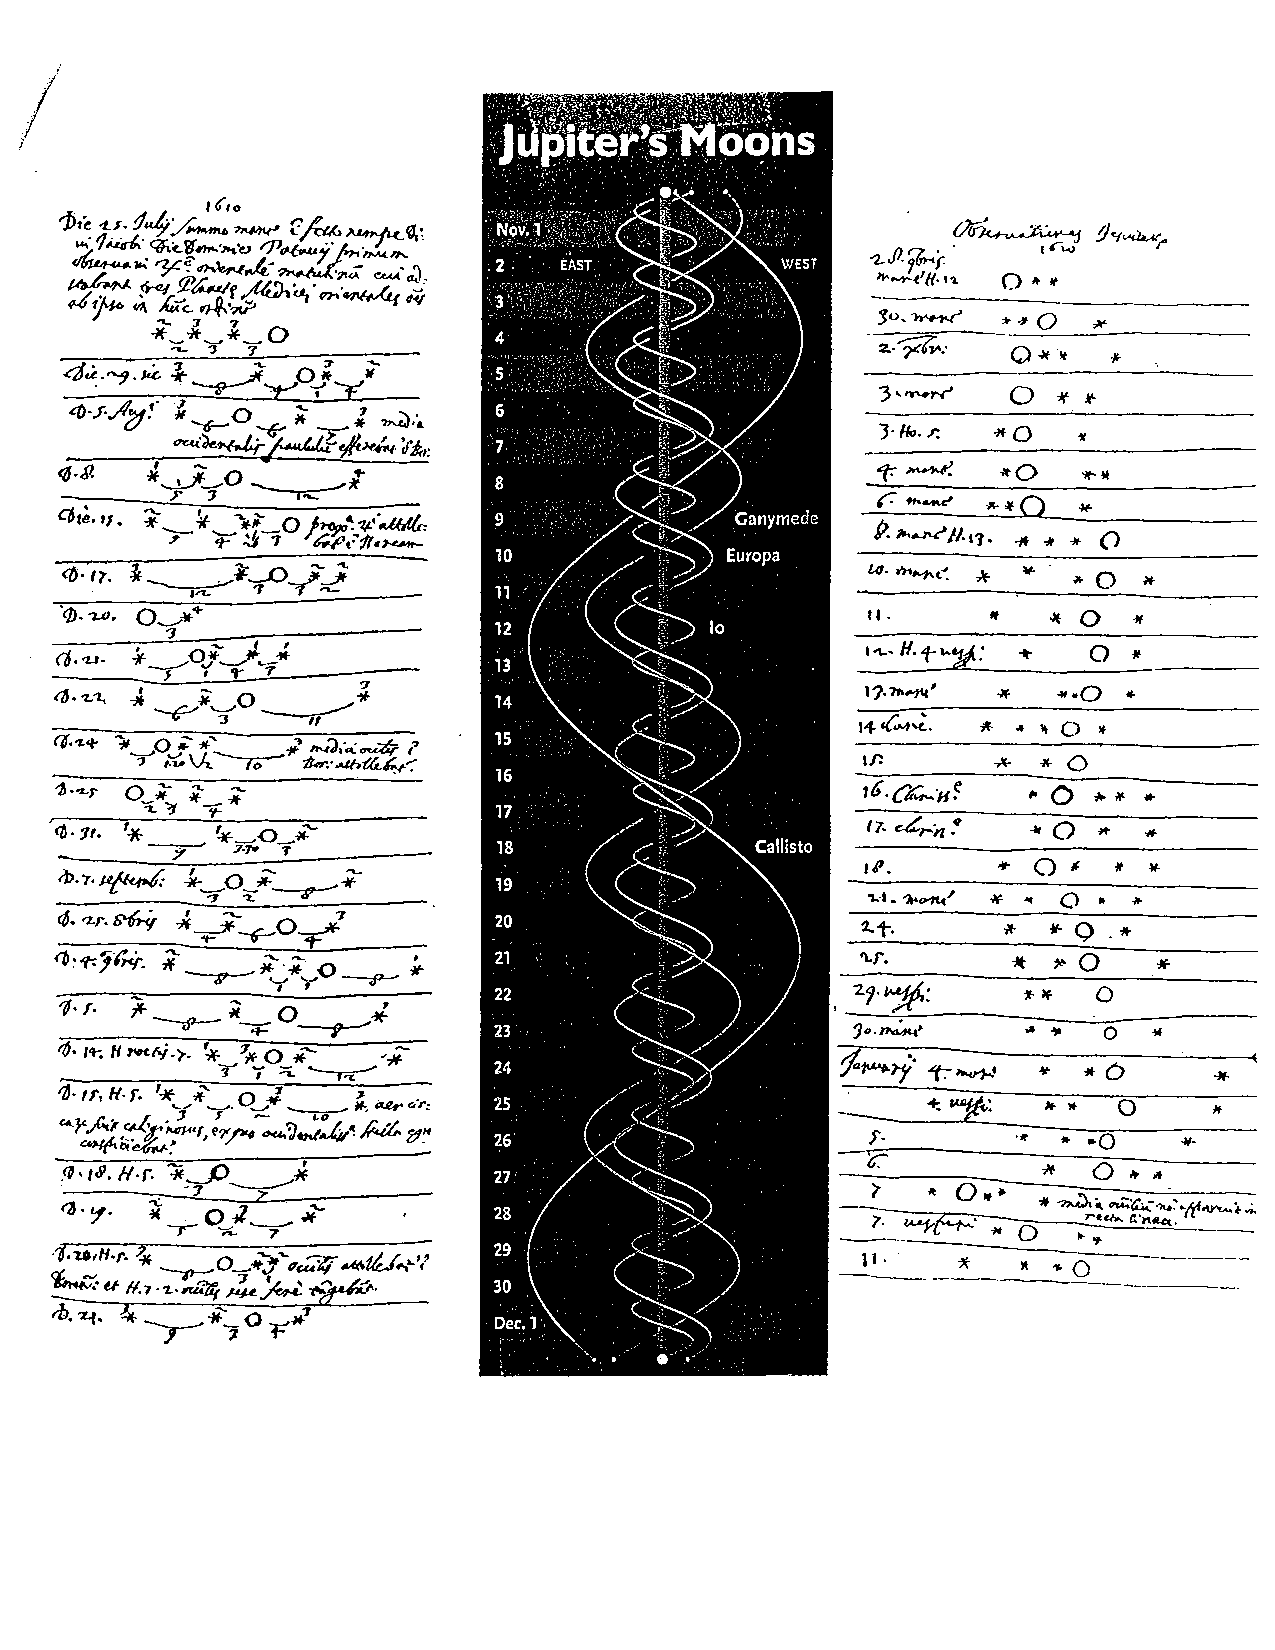
\includegraphics[width=\textwidth]{figures/problem-set-1-galileo-drawings.pdf}
\caption{Galileo's drawings of Jupiter and its satellites}
\end{figure}


\section{}

\begin{figure}[H]
\centering
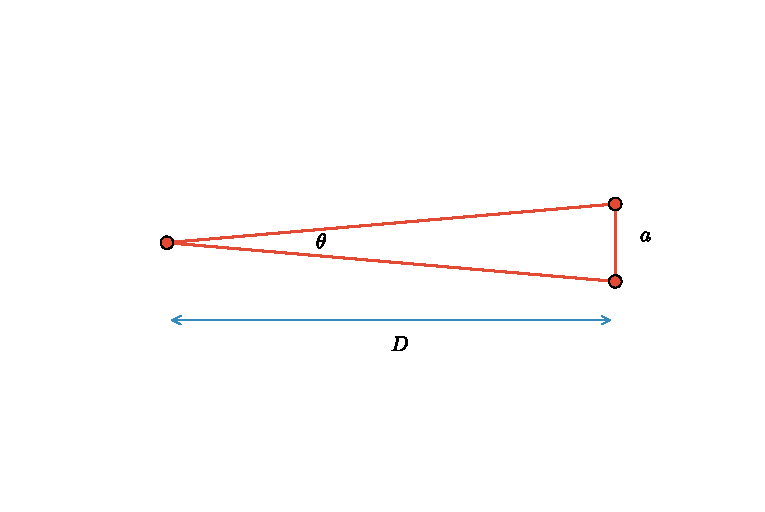
\includegraphics[width=\textwidth]{figures/problem-set-1-skinny-triangle.pdf}
\caption{Law of Skinny Triangles where $a = \theta \cdot D$.}
\end{figure}

Law of Skinny Triangles: $a = \theta \cdot D$. Here,

\begin{itemize}
\item $a =\ \text{Short Side} = \ \text{Diameter (physical of Saturn's rings)}$
\item $D = \ \text{Long Side} = \ \text{Distance to Saturn}$
\item $\theta = \ \text{Small angle (in rad)}$
\end{itemize}

Convert $\theta$ to radians:

\[\theta = 39\arcsec = \left(\pow{4.85}{-6}\frac{\rad}{\arcsec}\right) = \pow{1.89}{-4}\rad\]

\[D = \pow{1.3}{14}\cm = \ \text{Distance to Saturn}\]

Diameter of rings = $\theta \times D$ = $\left(\pow{1.89}{-4}\right) \times \left(\pow{1.3}{14}\right) \cm = a$. Then, $a = \pow{2.46}{10}\cm = 246,000\km$.




\end{document}
